\documentclass[mathserif,usenames,dvipsnames]{beamer}
\usepackage{algorithmic}
%\usetheme{Bergen}
%\usetheme{Copenhagen}
% \usetheme{Darmstadt}
% \usetheme{Frankfurt}
%\usetheme{Luebeck}
\usetheme{Madrid}
\usecolortheme{beetle}
%\usefonttheme{serif}
%\usecolortheme{dove}
%\usecolortheme{fly}
%\usecolortheme{seagull}
%\useinnertheme{rectangles}
%\useinnertheme{circles}
%\useinnertheme{inmargin}
%\useinnertheme{rounded}
%% =======================================================
%% (c) Tobias Schoofs
%% =======================================================
%% Commands 4 Programmers
%% =======================================================

%include lhs2TeX.fmt
%include lhs2TeX.sty

%\usepackage[pdftex]{graphicx}
%\usepackage{ucs}
%\usepackage[utf8x]{inputenc} 
\usepackage{tabto}
\usepackage[russian,portuguese,german,english]{babel}
\usepackage{CJK}
\usepackage{amsfonts}
\usepackage{amsfonts}

\usepackage{amsmath}
\usepackage{amssymb}
\usepackage{amsthm}
\usepackage{amscd}

\usepackage{siunitx}

\usepackage{listings}
\usepackage{longtable}

\usepackage{tikz}
\usepackage{pgfplots}

\usepackage{relsize}
\usepackage{xcolor}

\usepackage{soul}

\long\def\ignore#1{}

\newcommand{\acronym}[1]{\textsc{#1}}

\newcommand{\term}[1]{\textit{#1}}
\newcommand{\tech}[1]{{\ttfamily #1}}
\newcommand{\latin}[1]{\textit{#1}}
\newcommand{\speech}[1]{\textit{#1}}

\newcommand{\ie}{\textit{i.e.}}
\newcommand{\eg}{\textit{e.g.}}
\newcommand{\etc}{\textit{etc.}}
\newcommand{\viz}{\textit{viz.}}
\newcommand{\vs}{\textit{vs.}}

\newcommand{\sql}{\acronym{sql}}

\newcommand{\code}[1]{{\ttfamily #1}}
\newcommand{\cmdline}[1]{{\ttfamily #1}}

\newenvironment{sqlcode}{
\small
\begin{minipage}{\textwidth}
\lstset{language=sql,
        keepspaces=true,
        showspaces=false,
        showstringspaces=false}
}{
\end{minipage}
}

\newenvironment{python}{
\small
\begin{minipage}{\textwidth}
\lstset{language=python,
        keepspaces=true,
        showspaces=false,
        showstringspaces=false}
}{
\end{minipage}
}

\newenvironment{ccode}{
\small
\begin{minipage}{\textwidth}
\lstset{language=C,
        keepspaces=true,
        showspaces=false,
        showstringspaces=false}
}{
\end{minipage}
}

\newcommand{\keyword}[1]{\textbf{#1}}
\newcommand{\identifier}[1]{\textit{#1}}

\newcommand{\Rom}[1]{\uppercase\expandafter{\romannumeral #1\relax}}

\newcommand{\CC}{C\nolinebreak[4]\hspace{-.05em}\raisebox{.3ex}{\relsize{-2}{\textbf{++}}}}
\newcommand\csharp{C\nolinebreak[4]\hspace{-.02em}\raisebox{.3ex}{\relsize{-1}{\#}}}

\newcommand{\comment}[1]{\textcolor{red}{#1}}

\newcommand{\nowdb}{\textsc{n}o\textsc{wdb}}

\newcommand{\connect}[2]{
  \draw [-,color=black] (#1) to (#2)
}

% tikz
% \newcommand{\drawDataPoint}{\draw circle (0.2)}
% \drawDataGroup

% \renewcommand{\gcd}{\textsc{gcd}}

\title{Product Vision}
\author{Tobias Schoofs}
\begin{document}

% TITLE
\frame{\titlepage}

% WHAT
\begin{frame}
\frametitle{NoWDB}
\begin{equation*}
\nowdb = (graph +  timeseries + \acronym{sql} + Lua) \times Python
\end{equation*}
\begin{itemize}
\item A data processing platform
\item For large amounts of \term{timeserish} data
\item That can be used with standard interfaces (\acronym{sql})
\item Emphasising data science on client side
\item Emphasising big-data on server side
\end{itemize}
\end{frame}

% WHY TIMESERIES
\begin{frame}
\frametitle{Timeseries (1/2)}
\begin{itemize}
\item Growing amount of data are timeseries \emph{to some extent}
\item Important driver: \acronym{i}o\acronym{t}
\item But also: ``traditional'' industries:
      \begin{itemize} 
      \item \acronym{it} infrastructure providers,
      \item Energy,
      \item Manufacturing (``Industry 4.0''),
      \item Retail,
      \item Fintech,
      \item \dots
      \end{itemize}
\item Timeseries data have special requirements:
      \begin{itemize}
      \item Fast ingestion ($> 1M/s$)
      \item Scalability of queries ($> 1B metrics$)
      \item Special handling of time dimension
      \item Timeseries are less rigid compared to relational data\\
            (time points may be lost or duplicated)
      \end{itemize}
\end{itemize}
\end{frame}

\begin{frame}
\frametitle{Timeseries (2/2)}
\begin{columns}[T]
\column{0.75\linewidth}
\begin{itemize}
\item Avalailable timeseries databases are too narrow, 
      \ie\ \emph{pure} timeseries.
\item Examples:
      \begin{itemize}
      \item \acronym{i}nflux\acronym{db}
      \item \acronym{o}pen\acronym{tsdb}
      \end{itemize}
\item There are projects trying to solve this issue,
      \eg: \[
      timescale = relational + timeseries\]
      $\dots$ but it's still Postgres: somewhat slow
\end{itemize}
\column{0.25\linewidth}
\vskip1.0cm

\includegraphics[width=0.7\linewidth]{../img/influxlogo.png}\\[12pt]

\includegraphics[width=0.8\linewidth]{../img/tsdblogo.png}\\[12pt]
\vskip0.5cm

\includegraphics[width=0.8\linewidth]{../img/timescalelogo.png}
\end{columns}
\end{frame}

% WHY GRAPH
\begin{frame}
\frametitle{Graph}
\begin{columns}[T]
\column{0.75\linewidth}
\begin{itemize}
\item Make timeseries more widely applicable!
\item Natural candidates: Relational and Graph
\item Graph is more flexible:\\
      we can add new edges \\
      without changing the structure of entities
\item Graph is less rigid:\\
      duplicated edges are no issue
\end{itemize}
\column{0.25\linewidth}
\begin{center}
\vskip-0.4cm
\hskip-0.4\linewidth
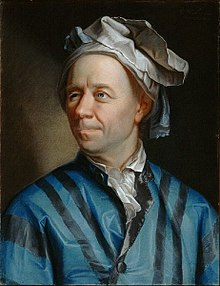
\includegraphics[width=0.75\linewidth]{../img/leoeuler.jpg}\\
\vskip-0.2cm
\hskip-1.2cm
{\tiny The Founder of Graph Theory:}
\vskip-0.2cm
\hskip-1.2cm
{\tiny Leonhard Euler}
\end{center}
\end{columns}
\begin{center}
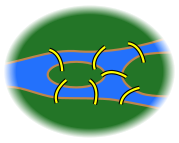
\includegraphics[width=0.25\linewidth]{../img/bridges1.png}
\raisebox{1cm}{\Huge $\rightarrow$}
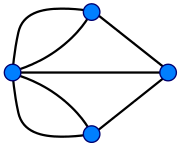
\includegraphics[width=0.25\linewidth]{../img/kgraph.png}
\end{center}
\end{frame}

% WHY Python
\begin{frame}
\frametitle{
\includegraphics[width=0.2\linewidth]{../img/pythonlogo.png}}
Provide full power of data-science tools on client side:
\begin{itemize}
\item NumPy
\item SciPy
\item Pandas
\item Matplotlib
\item \dots
\end{itemize}
Provide ready-made domain-specific packages:
\begin{itemize}
\item Statistics
\item Timeseries
\item Bayes, Support Vector Machines, Clustering, \etc\
\item Geodata
\item Retail (\eg\ recommendation engine)
\end{itemize}
\end{frame}

% WHY Lua
\begin{frame}
\frametitle{\raisebox{0.8cm}{\acronym{sql} +} 
\includegraphics[width=0.15\linewidth]{../img/lualogo.png}}
High level of integration client \& server:
\begin{itemize}
\item Server-side support for domain-specific packages,\\
      \ie\ support in \acronym{sql} and server-side scripting
      (Lua \& Python)
\item Stream Processing
\item Monitoring
\item Integration with messaging tools (\eg\ Kafka)
\item External Interfaces:
\begin{itemize}
\item native (Python, C, Go, \etc)
\item \acronym{rest} (for, \eg, Grafana)
\item \acronym{html} (through, \eg, Go)
\item \acronym{odbc/jdbc}
\end{itemize}
\end{itemize}
\end{frame}

% Strategy
\begin{frame}
\frametitle{Strategy}
\begin{itemize}
\item \textbf{Complement} existing \acronym{oltp} infrastructures
\item \textbf{Compete} with complex big-data and data science platforms
\item Provide a \textbf{low-cost} alternative 
      to frameworks with high cost of ownership
      (\eg: Hadoop, large \acronym{olap} systems, \etc)
\item Target industries with \textbf{timeserish} data 
      and need of data science
      (\eg\ \acronym{i}o\acronym{t}, retail, fintech, ``Industry 4.0'')
\item Provide pre-packaged out-of-the-box solutions
      (\eg\ integration with Kafka, Zookeeper, \acronym{spark} \& Grafana)
\item Operate with a mix of open-source and proprietary licenses
      (\eg\ generic modules for free, specific modules for pay)
\end{itemize}
\end{frame}
\end{document}
